\chapter{Background}
% A more extensive coverage of what's required to understand your work.

% In general you should assume the reader has a good undergraduate
% degree in computer science, but is not necessarily an expert in the
% particular area you've been working on. Hence this chapter may need to
% summarize some ``text book'' material.
%
% This is not something you'd normally require in an academic paper, and
% it may not be appropriate for your particular circumstances. Indeed,
% in some cases it's possible to cover all of the ``background''
% material either in the introduction or at appropriate places in the
% rest of the dissertation.
%

In this Chapter, I explain how scheduling works in Kubernetes. I will then
explain the concepts behind \textsc{Pronto}, as well as the reasons for exploring
\textsc{Pronto}'s application in Kubernetes. I will also describe related Kubernetes
schedulers. Finally, I will discuss the effectiveness of applying \textsc{Pronto}'s
algorithm within a Kubernetes system.

\section{Kubernetes}

\subsection{Kubernetes Overview}

\begin{figure}[H]
    \centering
    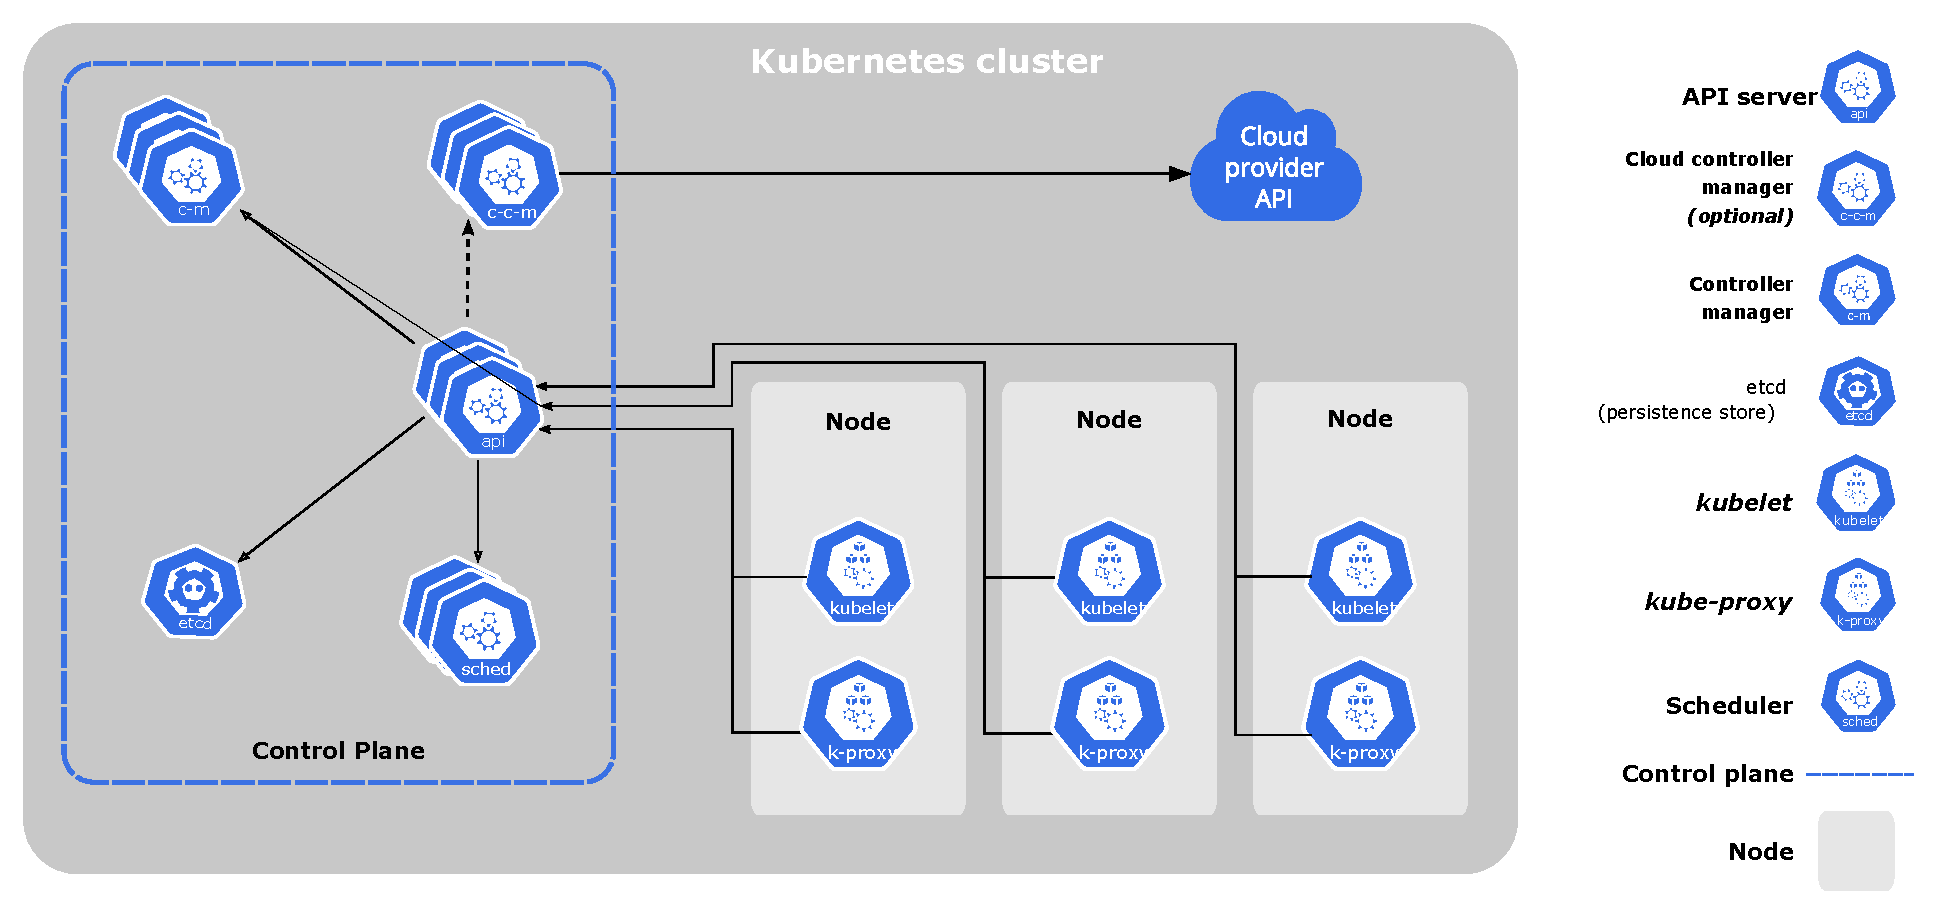
\includegraphics[width=\textwidth]{images/components-of-kubernetes.pdf}
    \caption{The components of a Kubernetes cluster
    \cite{kubernetes-components}}
    \label{kube-components}
\end{figure}

A Kubernetes cluster consists of a control plane and one or more worker Nodes.
Components in the control plane manage the overall state of the cluster. The
\verb|kube-apiserver| exposes the Kubernetes HTTP API, which is used to publish
objects such as Deployments, DaemonSets and Jobs. Each
Node in the cluster contains a \verb|kubelet| which manages Pods and ensures
they and their containers are running via a container runtime.

Kubernetes objects are persistent entities in the Kubernetes system. They act as
``records of intent" and describe the cluster's desired state: once created, the
Kubernetes system will constantly work to ensure that the objects exists. The
Kubernetes API is used to create, modify or delete these Kubernetes objects. Almost
every Kubernetes object includes two fields: \verb|spec| and \verb|status|.
\verb|spec| is used on creation as a description of the Objects desired state.
You can define affinities and QoS classes within this field. Containers also
contain a \verb|spec| field which specifies \verb|request| and
\verb|limits|. The \texttt{request} field behaves as a set of minimum
requirements and is used when scheduling Pods. In contrast, the \texttt{limits}
field is used by kernel of the Node to throttle a container's resource usage.
\verb|status| describes the current state of the object, supplied and updated by
the Kubernetes system. These fields are core to scheduling in Kubernetes.

\subsection{Scheduling in Kubernetes}
In Kubernetes, Pods are the smallest deployable units of computing that you can
create and manage in Kubernetes. It represents a single instance of a running
process in your cluster and typically contains one or more containers that are
tightly coupled and share resources. Pods can be individually created with their
own Yaml files. However, the Kubernetes API also provides workload objects to
manage multiple pods: these objects represent a higher abstraction level than a
Pod, and the Kubernetes control plane uses the workload's specification to
manage Pod objects on your behalf. Example workloads include Deployment,
StatefulSet, DaemonSet and Job.

When a Pod is created, it initially exists in a ``Pending" state - it has been
declared but hasn't yet been allocated to a Node. Kubernetes schedulers watch for
newly created but unassigned Pods, and based on a set of
rules or algorithms, select the most suitable Node for that Pod. Once a Node is
chosen, the scheduler ``binds" the Pod to the Node, updating the Pod's definition
in the Kubernetes API server by setting its \verb|spec.nodeName| field to the
name of the Node. Once this occures, the Pod transitions from ``Pending" to
``Running".

\section{\protect\textsc{Pronto}}

\subsection{Principle Component Analysis}
This section first explains Singular Value Decomposition (SVD) and how it
relates to solutions of Principal Component Analysis (PCA). I then introduce
Incremental-SVD and Subspace-Merge, which are used to perform FPCA on the stream
of telemetry produced by each Node.

\subsection{Singular Value Decomposition}
The SVF of a real matrix $\mathbf{A}$ with $m$ rows and $n$ columns where $m
\geq n$ is defines as $\mathbf{A} = \mathbf{U}\Sigma\mathbf{V}^T$, where $U$ and
$V$ are orthogonal matrices of shape $m \times m$ and $n \times n$ and $\Sigma$
is a rectangular matrix of shape $m \times n$ with singular values $\sigma_i$
along its diagonal \cite{}.
\begin{align}
\mathbf{A} = \begin{bmatrix} a_{11} & \dots & a_{1n} \\ \vdots & \ddots & \vdots
    \\ a_{m1} & \dots & a_{mn} \end{bmatrix} = \begin{bmatrix} \mid \\ u_1 \\
        \mid \end{bmatrix} \dots \begin{bmatrix} \mid \\ u_m \\ \mid
            \end{bmatrix} \begin{bmatrix} \sigma_1 & & \\ & \ddots & \\ & &
                \sigma_m \\ & 0 & \\ & & \\ & & 0 \end{bmatrix} \begin{bmatrix}
\text{---} & v_1^T & \text{---} \\ \vdots \\ \text{---} & v_m^T & \text{---} \\
\text{---} & v_{m+1}^T & \text{---} \\ \vdots \\ \text{---} & v_n^T & \text{---}
\end{bmatrix}
\end{align}

SVD can also be written compactly by discarding the elements which do not
contribute to $\mathbf{A}$.
\begin{align}
\mathbf{A} = \begin{bmatrix} \mid \\ u_1 \\ \mid \end{bmatrix} \dots
    \begin{bmatrix} \mid \\ u_m \\ \mid \end{bmatrix} \begin{bmatrix} \sigma_1 &
        & \\ & \ddots & \\ & & \sigma_m \end{bmatrix} \begin{bmatrix} \text{---}
& v_1^T & \text{---} \\ & \vdots & \\ \text{---} & v_m^T & \text{---}
\end{bmatrix}
\end{align}

There always exists the SVD for a real matrix, but the decomposition is not
unique: if $\mathbf{A} = \mathbf{U}_1\Sigma\mathbf{V}_1^T =
\mathbf{U}_2\Sigma\mathbf{V}_2^T$ then $\Sigma_1 = \Sigma_2$ but $\mathbf{U}_1 =
\mathbf{U}_2\mathbf{B}_a$ and $\mathbf{V}_1 = \mathbf{V}_2\mathbf{B}_b$ for some
block diagonal unitary matrices $\mathbf{B}_a, \mathbf{B}_b$ \cite{}. Each
column in $\mathbf{U}$ and $\mathbf{V}$ is an eignenvector of
$\mathbf{AA}^T$ and $\mathbf{A}^T\mathbf{A}$.

\subsection{Principal Component Analysis}
Pricipal Component Analysis is a staple of linear dimensionality-reduction
techniques. The standard PCA procedure takes as input a matrix $\mathbf{B}$
representing $n$ columns of data with $m$ dimensions. The matrix is first
mean-centered: $\mathbf{A}_{ij} = (\mathbf{B}_{ij} - \mu_i)$ where $\mu_i$ is
the mean of the row $i$. The output of PCA is a set of vectors that explain most
of the variance within $\mathbf{B}$. Given the covariance of a matrix
$\mathbf{A}$ is given as $\mathbf{AA}^T$ the Principal Components (PCs) maximise
the following equation:
\begin{align}
\text{Var}_i = \max_{\substack{x_i \in \mathbb{R}^m \setminus \{\mathbf{0}\} \\
    \|x_i\|=1 \\ x_i \perp x_1 \dots x_{i-1}}} x_i^T \mathbf{A} \mathbf{A}^T x_i
\end{align}

Given $\mathbf{A} = \mathbf{U}\Sigma\mathbf{V}^T$ from SVD,
$\mathbf{AA}^T = \mathbf{U}\Sigma\mathbf{V}^T\mathbf{V}\Sigma\mathbf{U}^T =
\mathbf{U}\Sigma^2\mathbf{U}^T$. Therefore, it can be shown that the PCs
$x_i = u_i$ from $\mathbf{U}$. The pair $\mathbf{U}, \Sigma$ will also be
referred to as a subspace as they provide sufficient information to describe the
orginal $\mathbf{B}$ matrix.

\subsection{Subspace-Merge}
Subspace-Merge is used to merge two subspaces together. Given two subsets
$(\mathbf{U}_1, \Sigma)$ and $(\mathbf{U}_1, \Sigma)$ from $\mathbf{Y}_1$ and
$\mathbf{Y}_2$ respectively, the subspace of $\mathbf{Y} = [\mathbf{Y}_1,
\mathbf{Y}_2]$ is:
\begin{align}
    \mathbf{U}\Sigma = \text{SVD}([\mathbf{U}_1\Sigma_1, \mathbf{U}_2\Sigma_2])
\end{align}
$[\mathbf{A}, \mathbf{B}]$ signifies the concatenation of two matrices with the
same number of rows.

\subsection{Incremental-SVD}
Incremental-SVD allows \textsc{Pronto} to become a streaming algorithm with limited
memory. It takes a stream of chunks $\mathbf{Y}_i$, such that  $[\mathbf{Y}_1,
\ldots, \mathbf{Y}_l] = \mathbf{Y}$, and with each recieved chunk it performs
Subspace-Merge to produce $\mathbf{U}_l, \Sigma_l$ where $\mathbf{Y} =
\mathbf{U}_l\Sigma_l\mathbf{V}_l^T$

\begin{algorithm}
\caption{Incremental-SVD}
\textbf{Data:} $\mathbf{Y} = [\mathbf{Y}_1, \dots, \mathbf{Y}_l]$ \\
    \textbf{Result:} $\mathbf{U}_l, \Sigma_l$ such that $\mathbf{Y} =
    \mathbf{U}\Sigma\mathbf{V}^T$
\begin{algorithmic}
\State $\mathbf{U}_1, \Sigma_1, \mathbf{V}_1^T = \text{SVD}(\mathbf{Y}_1)$
\For {$i = 2$ to $l$ do}
\State $\mathbf{U}_i, \Sigma_i, \mathbf{V}_i^T = \text{SVD}([\mathbf{U}_{i-1}\Sigma_{i-1}, \mathbf{Y}_i])$
\EndFor
\end{algorithmic}
\end{algorithm}
If the shape of the batches of data is $m \times b$, the space complexity of
Iterative-SVD is $\mathbb{O}(m^2 + mb)$ as only the latest version of
$\mathbf{U}_i,\Sigma_i$ and $\mathbf{Y}_i$ are needed for each iteration.

\subsection{FPCA and FSVD}
FPCA combines the relationship between standard SVD and PCA with the
Subspace-Merge operation, to calculate the PCs of the data $[\mathbf{Y}_1,
\ldots,\mathbf{Y}_m]$ from $m$ nodes. Every node $i$ performs perform SVD  on
their local data, to produce the subspace $\mathbf{U}_i, \Sigma_i$. These
subspaces can be merged using at most $m-1$ Subspace-Merges to obtain the global
subspace $\mathbf{U}'\Sigma'$, corresponding to the PCs of the aggregated data
from all the nodes. \textsc{Pronto} turns this procedure into a streaming algorithm, by
running Subspace-Merge on the subspaces produced by incremental-SVD. Finally,
\textsc{Pronto} also introduces a forgetting factor $\gamma$ in front of
$\mathbf{U}_i\Sigma_i$ in Incremental-SVD that gradually reduces the influence
of previous subspaces. Like with standard PCA, FPCA can be considered as FSVD on
centered data.

\subsection{Low-Rank Approximations}
It can be shown that using the first $r$ eignenvectors in the above algorithms
approximate the result of using all $m$ eignenvectors, i.e. if
\begin{align}
\mathbf{Y} = \begin{bmatrix} \mid & & \mid \\ u_1 & \ldots & u_m
    \\ \mid & & \mid  \end{bmatrix} \begin{bmatrix} \sigma_1 &
        & \\ & \ddots & \\ & & \sigma_m \end{bmatrix} \begin{bmatrix} \text{---}
& v_1^T & \text{---} \\ & \vdots & \\ \text{---} & v_m^T & \text{---}
\end{bmatrix}
\end{align}
We can use $\mathbf{U}^r = \begin{bmatrix} \mid & & \mid \\ u_1 & \ldots & u_r
    \\ \mid & & \mid  \end{bmatrix}$ and $\mathbf{\Sigma}^r = \begin{bmatrix}
\sigma_1 & & \\ & \ddots & \\ & & \sigma_r \end{bmatrix}$ where $r \leq m$ in
Incremental-SVD and Subspace-Merge. This lets \textsc{Pronto} reduce the number of
computations it performs and its memory usage.

\subsection{\protect\textsc{Pronto} System Overview}
\begin{figure}[H]
    \centering
    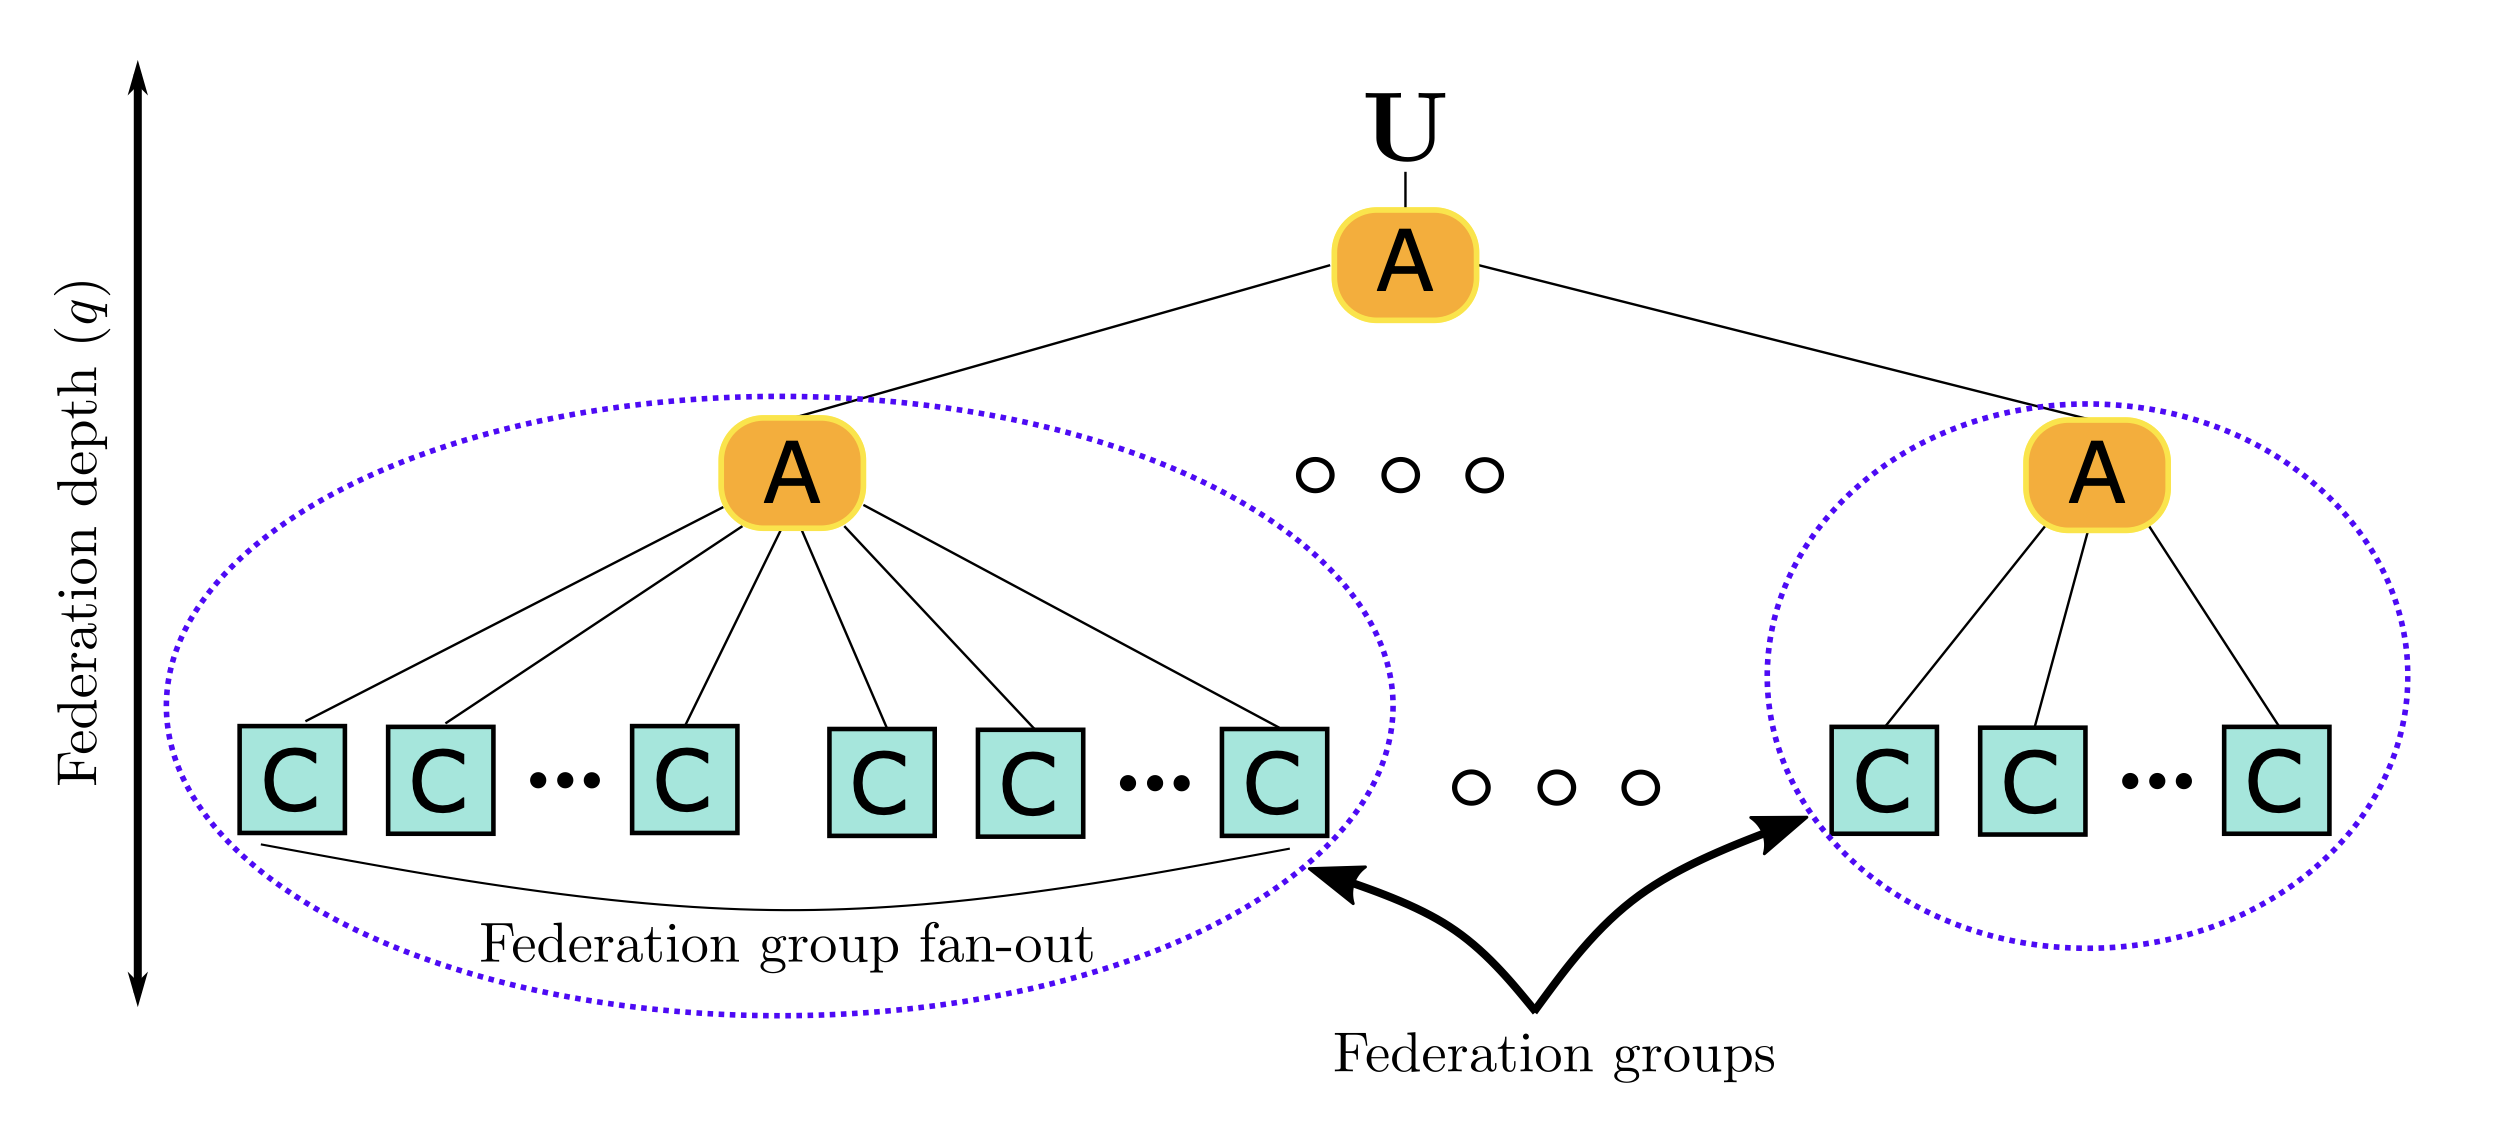
\includegraphics[width=\textwidth]{images/pronto-agg.png}
    \caption{How local models are aggregated in \textsc{Pronto}. Dedicated aggregator
    nodes propagate the updated subspaces until the root is reached
    \cite{grammenos_pronto_2021}.}
    \label{pronto-agg}
\end{figure}
There are two types of nodes in \textsc{Pronto}: compute node (C) and aggregator node
(A). Compute nodes collect and center node statistics (i.e. CPU and Memory) and
perform Incremental-SVD to obtain the low rank approximations of the local
subspace $\mathbf{U},\Sigma$. The aggregator nodes before Subspace-Merge on
incoming subspaces, with subspace produced by the root aggregator node being
propagated back to the compute nodes.

\subsection{\protect\textsc{Pronto} Reject-Job Signal}
\begin{figure}[H]
    \centering
    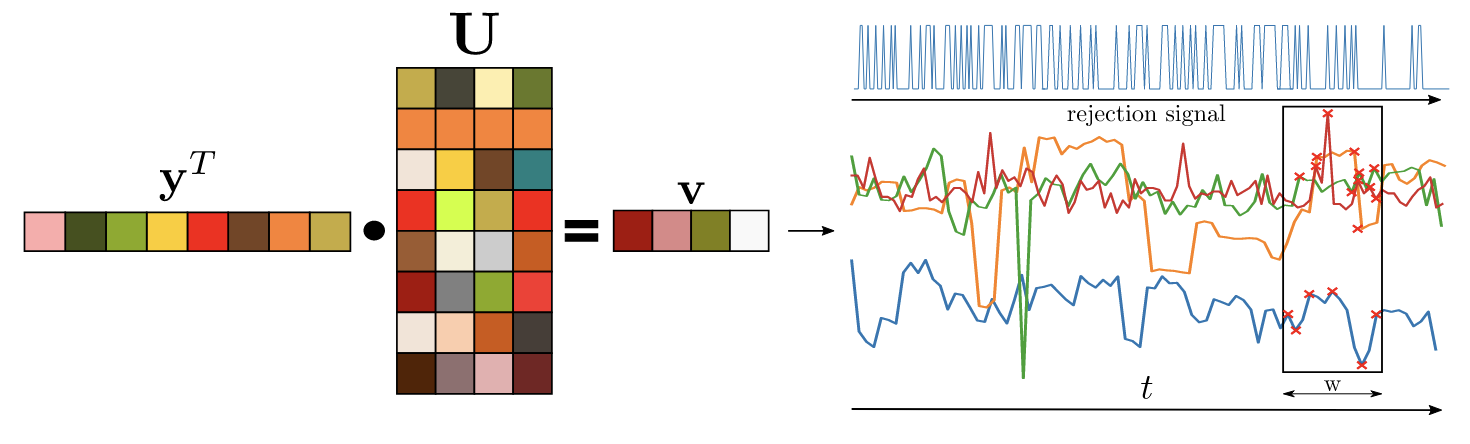
\includegraphics[width=\textwidth]{images/pronto}
    \caption{Projection of incoming $y \in \mathbb{R}^d$ onto embedding $U \in
    \mathbb{R}^{d \times r}$ producing $R$ projections in $v \in \mathbb{R}^{1
    \times r}$. Projections are tracked over time for detecting spikes which
    form the basis of the rejection signal. The sliding window for spike
    detection for each projection is of size $w$ also shown in the figure.}
    \label{pronto-components}
\end{figure}

Each compute node projects their data onto the latest version of $\textbf{U}$,
and identifies all the spikes. If the weighed sum of these spikes, using the
corresponding singular values in $\Sigma$, exceeds a threshold, a rejection
signal is raised to indicate that the node is potentially experiencing
performance degradation and a job should not be scheduled on that node.

\subsection{Strengths}
\textsc{Pronto}'s ability to accurately predicting spikes in traces from real-world
datacenters was compared against non-distributed dimensionality-reduction
methods \cite{}, \textsc{Pronto}'s improved performance over the non-distributed
strategies implies that there were correlations between job's resource usages on
different nodes at the same point in time. This suggested that FPCA could use
telemetry across multiple nodes to more acurrately compute the principle
components and thus could more accurately predict performance degradation.
These results also indicated a potential benefit from applying \textsc{Pronto} to a
Kubernetes environment.

\subsection{Weaknesses}
\subsubsection{Assumptions}
The Pronto paper only provides a method with which to measure node
"responsiveness" to future workloads. However, it does not include an allocation
algorithm which then uses this scoring. Furthermore, a binary signal makes it
difficult to score nodes against each other. Other schedulers typically use a
scoring function to pick the "optimal" node \cite{kube-scheduler}\cite{}.

In addition, the paper makes multiple assumptions which don't hold in a Kubernetes
scheduler. Firstly, it assumes there is no communication latency within the system.
This also implicitly assumes no binding latency: no latency between a node
accepting a task and the task starting to run on the node. This is important as
the spike prediction uses live telemetry data to predict spikes, and thus the
score only considers currently running task. In Kubernetes, the latency between
a pod being bound to a node and the pod actually running on the node is
significant \cite{tyczynski_kubernetes_2015}. This introduces another challenge to directly applying
Pronto to Kubernetes, as nodes may accept too many pods as the signal does not
reflect the "in flight" pods.

% The Pronto paper implements a binary "responsiveness" signal which predicts
% upcoming performance degradation. Because the authors assume a system with no
% communication latency (implicitly assuming that scheduled workloads were
% immediately visisble in the signal as well), they could send this signal
% directly to a central scheduler which could then stop assigning workloads once a
% node sent a Reject Signal.
%
% However, due to significant pod startup latency, the method can't be used in a
% real-world Kubernetes cluster is infeasible. When measuring pod startup in a
% 100 node clusters, the more than 50\% of pods took more than $\approx$ 1 second
% to startup. In addition, when nodes were 100\% full, pod startup could reach up
% to 4 seconds. This latency is significant when Kubernetes schedulers can
% support a throughput of $\approx$1000 pods per second
% \cite{qadeer_scaling_2022}. Applying the same approach as used in the paper,
% could result in nodes advertising a "willingness" to take on new pods while
% a large number of pods are in "flight" and once running will immediately
% overload the node. To prevent this runaway train type problem, I need to define
% a reservation function: a function that reserves an amount of the signal for a
% bound pod. This is necessary to allow previous scheduling decisions to have an
% imnpact on the signal while the signal updates to take into account the
% scheduled pods.
%
% In addition, telemetry-based schedulers can use individual node performance
% information to score and fine-tune pod allocations. A binary signal does not
% provide the necessary information for scoring nodes, potentially resulting in
% worse pod allocations.
%
% In summary, the requirements of the signal are:
% \begin{itemize}
    % \item Reservable: the scheduler must be able to track the pending impact of
        % previous scheduling decisions until the pods have begun running.
    % \item Comparable: the signal must provide enough information to score nodes
% \end{itemize}

\subsubsection{Peak-Prediction}
While CPU-Ready is specific to VMware vSphere, other contention metrics
are available on a Linux-based system. The closest related metrics are the
pressure stall information (PSI) metrics: pressure information for each resource
is exported through their respective file in
\verb$/proc/pressure/<cpu|memory|io>$. Within each file, the metrics are
broken down into two categories: some - which indicates the share of time in
which at least some tasks are stalled on a given resource, and full which
indicates the share of time in which all non-idle tasks are stalled on a given
resource simultaneously.

Pronto performs peak-detection on the metrics to predict future spikes which
then indicate high-resource contention and degraded performance. Therefore, for
Pronto to make accurate predictions and produce a correct RejectJob signal, PSI
must exhibit spikes during high-resource contention. To investigate the
feasibility of peak prediction within a Kubernetes node using PSI metrics, I
polled the \verb|/proc/pressure| files of nodes when under different workloads.

\begin{figure}[htbp!]
    \centering
    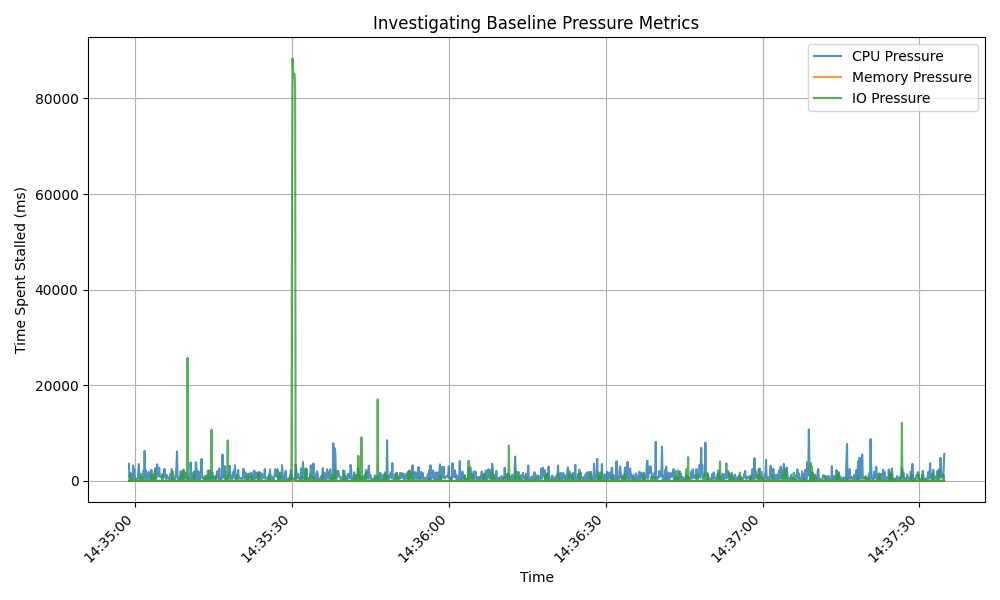
\includegraphics[width=0.48\textwidth]{images/pressure-baseline.png}
    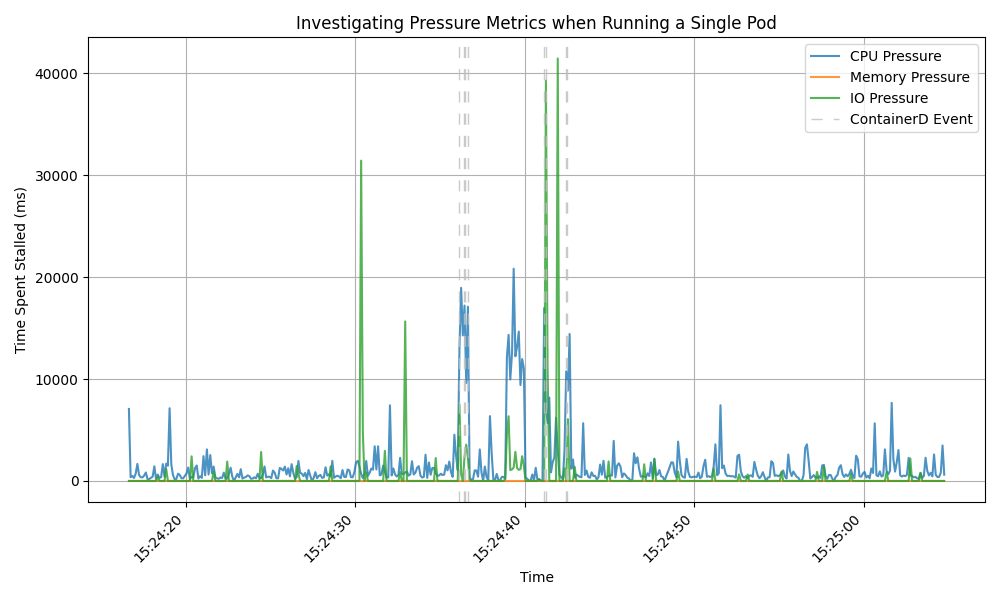
\includegraphics[width=0.48\textwidth]{images/pressure-single.png} \\
    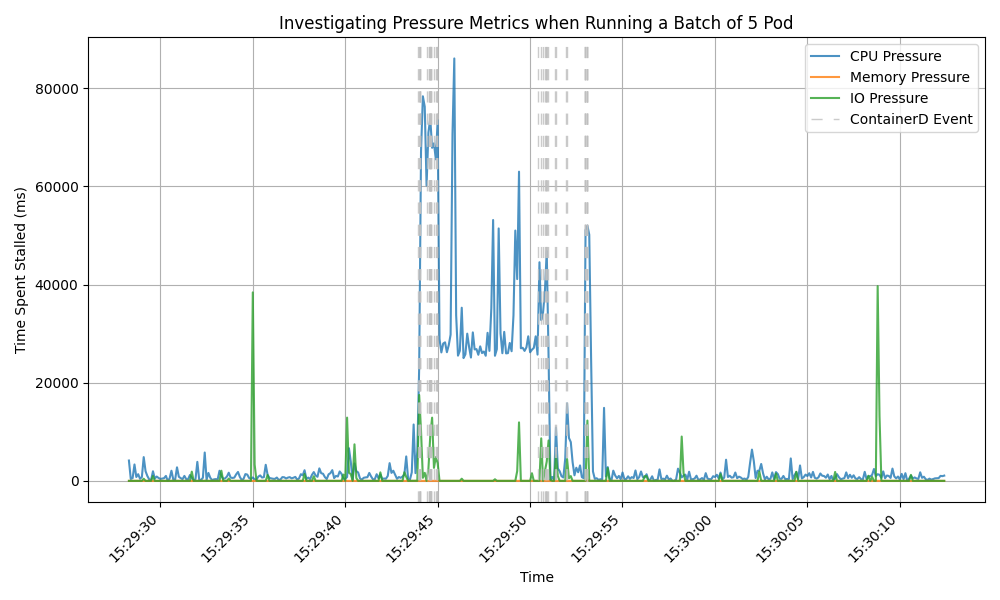
\includegraphics[width=0.48\textwidth]{images/pressure-smallbatch.png}
    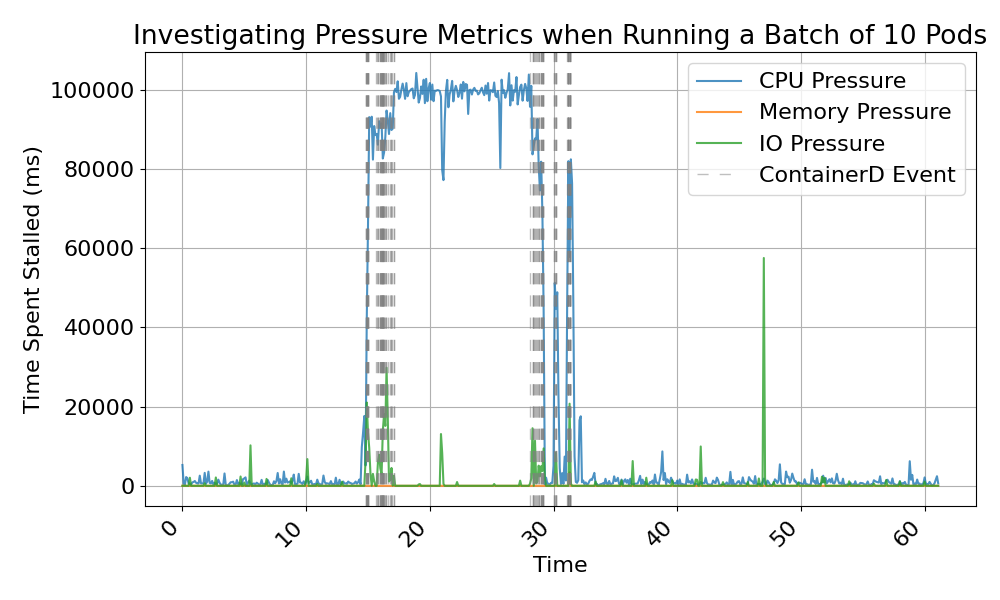
\includegraphics[width=0.48\textwidth]{images/pressure-bigbatch.png}
    \caption{Measurements of \texttt{/proc/pressure/} \texttt{total} value under
    different loads. The container runtime results in spikes no matter the
    workload.}
    \label{fig:pressure}
\end{figure}

From figure \ref{fig:pressure}, we can see how even with lightweight workloads,
the PSI metrics experience a spike in value. These spikes are due to the
container runtime, in this case Containerd, using resource to create or delete
the containers of the pods.

The PSI metrics also expose an average over the last 10 seconds.
\begin{figure}[htbp!]
    \centering
    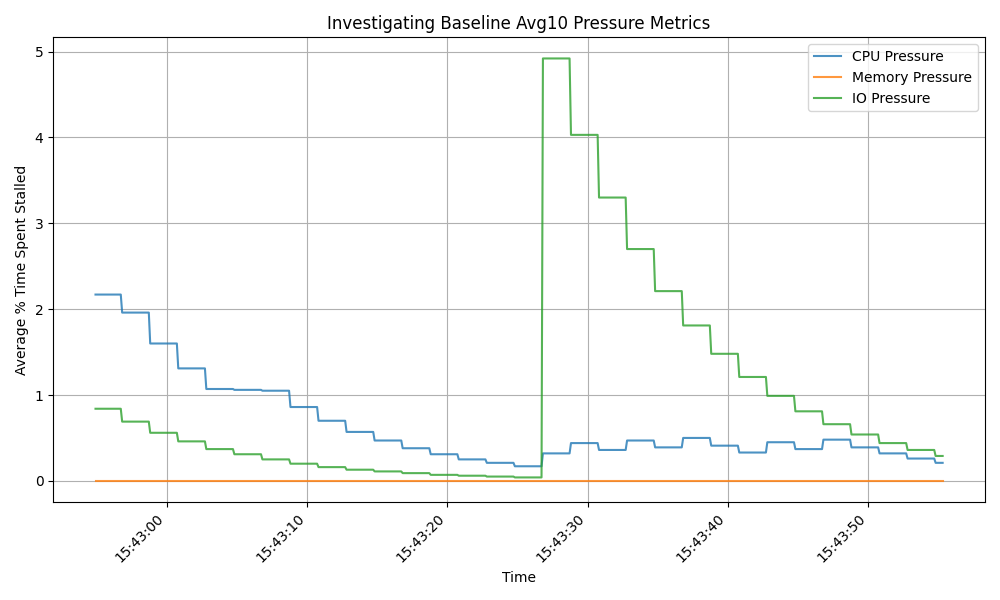
\includegraphics[width=0.48\textwidth]{images/avg-pressure-baseline.png}
    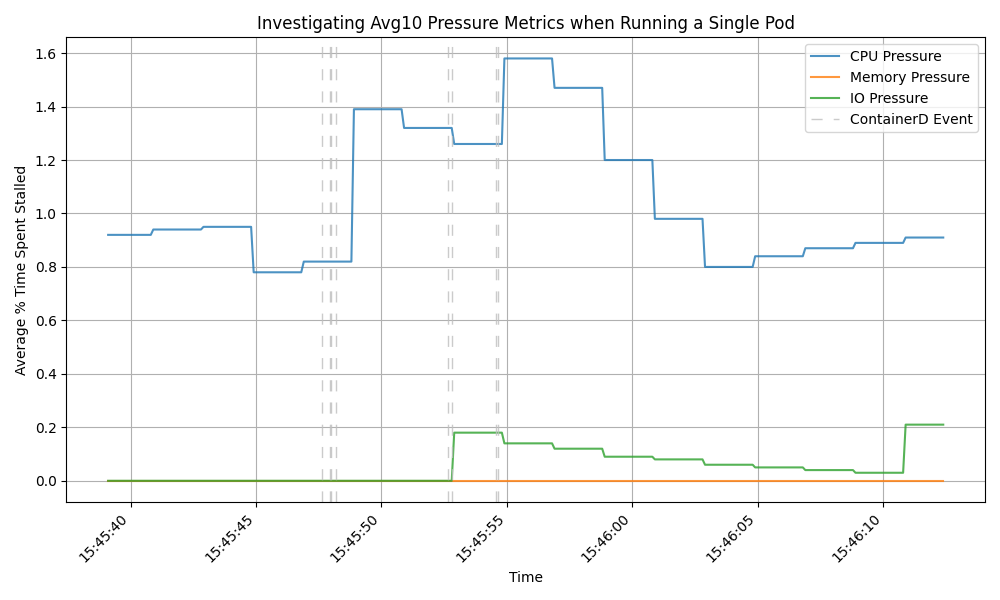
\includegraphics[width=0.48\textwidth]{images/avg-pressure-single.png} \\
    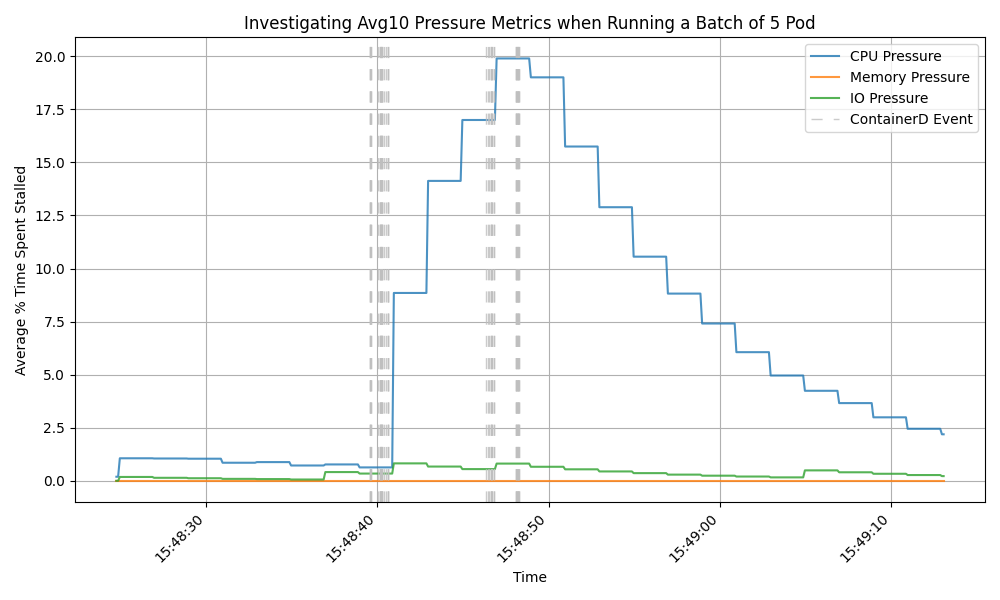
\includegraphics[width=0.48\textwidth]{images/avg-pressure-smallbatch.png}
    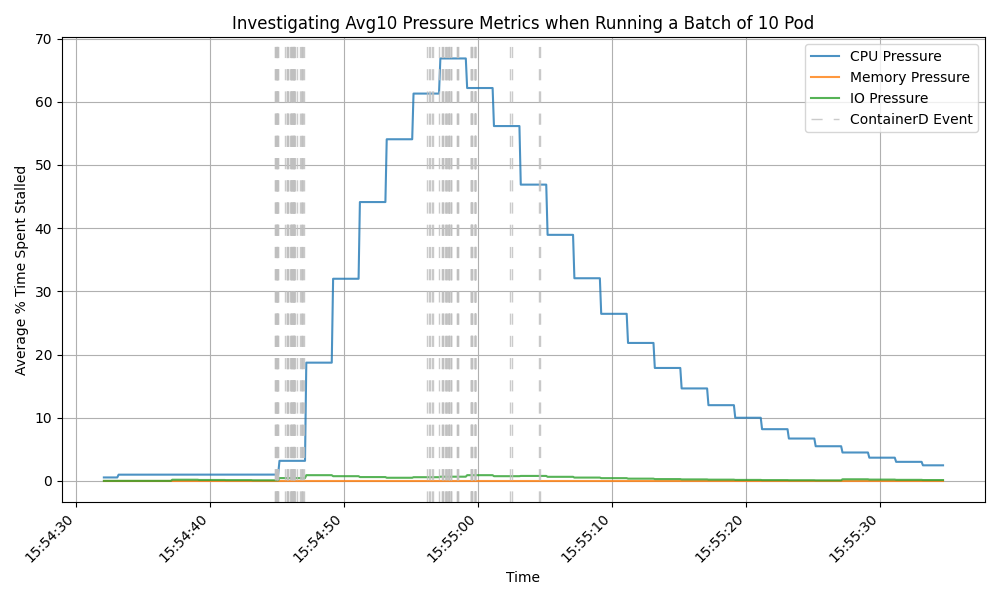
\includegraphics[width=0.48\textwidth]{images/avg-pressure-bigbatch.png}
    \caption{Measurements of \texttt{/proc/pressure/} \texttt{avg10} value
    under different loads. The container runtime results in spikes no matter the
    workload.} \label{fig:pressure-avg}
\end{figure}
Figure \ref{fig:pressure-avg} shows how the averaged value is able to reduce the
contention spikes. However, it also reduces the responsiveness of the metrics -
in the 10 pod batch, the metrics fails to rise to the same value as in the
total case before the pods have completed. From this investigation, I concluded
that peak-prediction with sub-second polling is not feasible within Kubernetes.

% In the paper, Pronto uses \verb|CPU-Reeady| which is generated by the VMware
% vSphere virtualisation platform. This metric can't be used within a
% Kubernetes cluster as machines can be both virtual and physical. Since Linux
% 4.20+, the kernel can track how long tasks are stalled waiting for the CPU
% at a cgroup granularity. By inspecting the the root cgroup’s CPU pressure
% file using \verb|cat /proc/pressure/cpu| you can measure the total time all
% processes spent waiting for the CPU to be available.
%
% While this type of metric can be used to alert of performance degradation,
% this metric has a few shortcomings. Firstly, it only reports CPU-centric
% information. This is not always representative measure of resource
% contention as memory-heavy workloads may starve for RAM resources while
% metrics like \verb|CPU-Ready| and \verb|/proc/pressure/cpu| remain
% unaffected.
%
% Secondly, a significant amount of resources are used starting up or deleting
% containers. This results in large spikes, as shown in figure
% \ref{pressure-eval}, which are difficult to distinguish from genuine CPU-Ready
% spikes. As Pronto uses spike detection to predict future resource performance
% degradation, container start-ups could produce detectable spikes which would
% reduce the rate at which pods are assigned to nodes and could result in lower
% throughput.
%


\section{Related Work}
In this section, I explore the existing Kubernetes scheduler space, identifying
those that share properties with \textsc{Pronto} and highlighting their strengths and
weaknesses.

\subsection{Telemetric-based Schedulers}

\subsection{Federated Schedulers}

\subsection{Reinforcement Learning Schedulers}

\subsection{Summary of Related Work}
The earlier survey compared how existing Kubernetes schedulers used two
difference classes of input data - static pod information and telemetry - to
guide their scheduling decisions. Pod description-based scheduling ensures that
fundamental resource guarantees are respected. Telemetry-based scheduling can
more precisely allocate pods to nodes at the cost of increased complexity.
Hybrid schedulers combine these methods to provide guarantees of fundamental
resource requests while fine tuning scheduling decisions. However, their
reliance on predefined pod requirements still limits the QoS they can achieve.
Without careful consideration and engineering, erroneous pod resource requests
can result in under-utilisation or high resource contention.

\section{Summary}

This chapter introduced the core concepts of online scheduling and the
Kubernetes environment. I explored existing Kubernetes schedulers, investigating
the merits of using pod description-based schedulers vs. telemetry-based
schedulers. From the brief survey, I identified that few Kubernetes schedulers
use deeper contention indicators, such as cache pressure and memory pressure.
A potential technique that could be applied to Kubernetes scheduling is Pronto:
a novel scoring method that uses a federated approach with contention-based
metric - allowing it to quickly predict performance degredation while catering
for distributional shifts. While Pronto can't be directly applied to Kubernetes,
its federated apsect and its use of contention-based metrics can inspire a new
FL approach.

% \begin{tcolorbox}[boxsep=0mm,left=2.5mm,right=2.5mm]
    % \textbf{Summary:} {\em In this chapter I will summarise the problem and
    % problem space. I will review the findings of the related work, highlighting
    % weaknesses of existing Kubernetes schedulesr with respect to QoS
    % scheduling.}
% \end{tcolorbox}

